
%   ------------------------------------------------------------------
%   ------------------------------------------------------------------
%                 Chapter set editing
%   ------------------------------------------------------------------
%   ------------------------------------------------------------------

\chapter{Use cases}

In all this use cases, the folder contains a file {\tt Info.txt} tha contains a list of
all commands plus some brief commentary.

%   ------------------------------------------------------------------
%   ------------------------------------------------------------------
%   ------------------------------------------------------------------

\section{Image devlopment}

%   ------------------------------------------------------------------
\subsection{Introduction/presentation}

This data set present a use-case for creation a devloped surface.  A detailled
description of the MMVII-command can be found in chapter~\ref{Chap:Mesh}.
The data, located in folder {\tt DevlopImage}  is made of $74$ images that correspond to a stereoscopic
acquisition of a map that present high, but smooth, deformation.


For the purpose of limitating the size in github, the images have been articifially
reduced of a factor $4$. Also the image have been made in non professional
condition with natural ligthing. Globally, the quality of the result is
not representative of what can be obtained by such tools.

A file {\tt Info.txt} contains the list of all command used, somes are in
comment.
At several step of the process, the pipeline requires some input of the user
(for example $2d$ and $3d$ masq).  To assure the reproductability, the 
data set provide a copy of the input that was made in floder {\tt DataAux}. 
In this case, in the file {\tt Info.txt}  the interactive command is commented, and subsitued
by a shell command that copy the data, for example :

\begin{itemize}
    \item for seizing the $3d$ masq, the command {\tt"mm3d SaisieMasqQT AperiCloud\_Basc.ply"}
	    is indicated but commented;
    \item to execute the process, the command {\tt "cp DataAux/AperiCloud\_Basc\_* ."} is indicated.
\end{itemize}

At this step, the pipeline is a mix of {\tt mmv1} and {\tt MMVII}. We give a fast description
of the {\tt mmv1} part as it is a classical pipeline and let the reader find more details
in the $500$ pages of the  {\tt mmv1} documentation.


%   ------------------------------------------------------------------

\subsection{The  {\tt mmv1} part}

The  {\tt mmv1} goes until the obtention of $3d$ mesh that describe the surfaces and
pose estimation of camera in the same repair.

     %   -  -  -  -  -  -  -  -  -  -  -  -  -  -  -  -  -  -  -  -  -  -  -  -

\subsubsection{Camera pose and calibration}

As the reduction has supressed the {\tt xif} meta-data, we indicate it
for {\tt mmv1}, the folder contains a file :

\begin{itemize}
    \item {\tt MicMac-LocalChantierDescripteur.xml}
\end{itemize}

We compute tie-point using {\tt @SFS} because of low contrast :

\begin{itemize}
    \item {\tt mm3d Tapioca MulScale ".*jpg" 400 1500 @SFS}
\end{itemize}

We compute orientation and calibration : 

\begin{itemize}
   \item {\tt Tapas FraserBasic "P.*jpg" Out=AllRel}
\end{itemize}

For  this pipeline, it's not absolutely necessary to be in a physicall repair,
but that's a good use to have ... We can seize the information with
{\tt SaisieBasc} and {\tt SaisieMasqQT}, replaced here by {\tt cp} from {\tt DataAux} . 
Once done we use :

\begin{itemize}
    \item {\tt mm3d SBGlobBascule P.*jpg Ori-AllRel/ MesBasc-S2D.xml Basc  PostPlan=Plan DistFS=10}
\end{itemize}

     %   -  -  -  -  -  -  -  -  -  -  -  -  -  -  -  -  -  -  -  -  -  -  -  -

\subsubsection{Computation of $3d$ model}

We must first create a $3d$ masq of the zone that will be used at different step .
We first create a sparse cloud for seizing :

\begin{itemize}
	\item {\tt AperiCloud "P.*jpg" Ori-Basc/}
\end{itemize}

After we can use {\tt mm3d SaisieMasqQT AperiCloud\_Basc.ply}, 
replaced here by a {\tt cp} from {\tt DataAux}.
Then we compute the $3D$ dense cloud :

\begin{itemize}
	\item {\tt mm3d C3DC BigMac P.*jpg Ori-Basc/ Masq3D=AperiCloud\_Basc\_selectionInfo.xml}
\end{itemize}

Finaly, we transform it in a $3d$ mesh :

\begin{itemize}
	\item {\tt TiPunch C3DC\_BigMac.ply Filter=0}
\end{itemize}

%   ------------------------------------------------------------------

\subsection{The  {\tt MMVII} part}

     %   -  -  -  -  -  -  -  -  -  -  -  -  -  -  -  -  -  -  -  -  -  -  -  -

\subsubsection{Inporting the data}

In the {\tt MMVII} part we need the pose of camera and the $3D$ mesh. The $3d$ mesh is 
in the standard  {\tt ply} format that is supported by  {\tt MMVII}, so there is nothing
to do. For the importing the orientation  we can use :

\begin{itemize}
	\item {\tt MVII OriConvV1V2 Ori-Basc/ Basc}
\end{itemize}

Curious reader, can inspect the folder {\tt MMVII-PhgrProj/Ori/Basc/}.

     %   -  -  -  -  -  -  -  -  -  -  -  -  -  -  -  -  -  -  -  -  -  -  -  -

\subsubsection{Correcting and filtering the mesh}

We use the command {\tt MeshCheck} and {\tt MeshCloudClip}, the first one
correct some topologicall probleme in the mesh, the second one restric
the mesh to our usefull zone  (because the poisson algorithm used in {\tt TiPunch}
create undesirable extensions) :

\begin{itemize}
	\item {\tt MMVII  MeshCheck C3DC\_BigMac\_mesh.ply Out=Correc-C3DC\_BigMac\_mesh.ply Bin=1}

	\item {\tt MMVII  MeshCloudClip Correc-C3DC\_BigMac\_mesh.ply  AperiCloud\_Basc\_polyg3d.xml}
\end{itemize}

     %   -  -  -  -  -  -  -  -  -  -  -  -  -  -  -  -  -  -  -  -  -  -  -  -

\subsubsection{Devlopment of the mesh}

Now we run the "kernel" algorithm to create the $2d$ development of the mesh :

\begin{lstlisting}
MMVII MeshDev Clip\_Correc-C3DC\_BigMac\_mesh.ply 
\end{lstlisting}

This command generate $2$ mesh :

\begin{itemize}
	\item {\tt Dev2D\_Clip\_Correc-C3DC\_BigMac\_mesh.ply} which is the devlopped surface itself,
              if may contain less triangle/point that the $3d$ intial mesh when this one is badly connected 
		
	\item {\tt Dev3D\_Clip\_Correc-C3DC\_BigMac\_mesh.ply} which is a subset of the $3D$ initial mesh
		that correpond to the $2D$ devlopped mesh (it will be equal to initial when there is no connectivity problem);
\end{itemize}

     %   -  -  -  -  -  -  -  -  -  -  -  -  -  -  -  -  -  -  -  -  -  -  -  -

\subsubsection{Computing visibility, quality , radiometry of triangles}

We now run the command  {\tt MeshProjImage} to prepare the texture mapping : this command
compute the visibility of each triangle in each image, it also computes tie points with 
radiometry to compute radiometric equalisation 

\begin{itemize}
    \item {\tt MMVII MeshProjImage "P.*jpg"  Dev3D\_Clip\_Correc-C3DC\_BigMac\_mesh.ply Basc DEV OutRadData=R0}
\end{itemize}

The parameter {\tt DEV} indicates where the data must be stored.
The parameter {\tt OutRad=R0} indicate that data for radiometry 
must be compute, and fix the folder where these data must be stored.

     %   -  -  -  -  -  -  -  -  -  -  -  -  -  -  -  -  -  -  -  -  -  -  -  -

\subsubsection{Equalizing the radiometry}

For radiometric equalization, we must know the aperture used for each image,
as the vignettage is dependand of aperture. As these images contains no metadata,
we must indicate it . This has to be indicated in the file :

\begin{itemize}
    \item {\tt MMVII-PhgrProj/MetaData/Std/CalcMTD.xml}
\end{itemize}

We can do it by copying the file {\tt DataAux/CalcMTD.xml}. We can also
do it using the command {\tt EditCalcMTDI} :

\begin{itemize}
      \item {\tt MMVII  EditCalcMTDI Std Aperture "Modif=[P.*.jpg,11,0]"  Save=1}
\end{itemize}

We must first create the initial radiometric model  we want to use, here we select
a degree $2$ by image :

\begin{itemize}
	\item {\tt MMVII RadiomCreateModel P.*jpg Init2 Basc DegIma=2}
\end{itemize}

Now we can compute the radometric equalization model :

\begin{itemize}
	\item {\tt MMVII RadiomComputeEqual P.*jpg R0 Init2 Equal Basc}
\end{itemize}


     %   -  -  -  -  -  -  -  -  -  -  -  -  -  -  -  -  -  -  -  -  -  -  -  -

\subsubsection{Map the texture}

And finally, we can create the devloped surface :


\begin{itemize}
	\item {\tt MMVII MeshImageDevlp Dev2D\_Clip\_Correc-C3DC\_BigMac\_mesh.ply  DEV InRadModel=Equal}
\end{itemize}

The results can be found in {\tt MMVII-PhgrProj/MeshDev/DEV/DevIm.tif}, an illustration is shown on figure~\ref{fig:TutDI:DevIm}.


\begin{figure}
\centering
	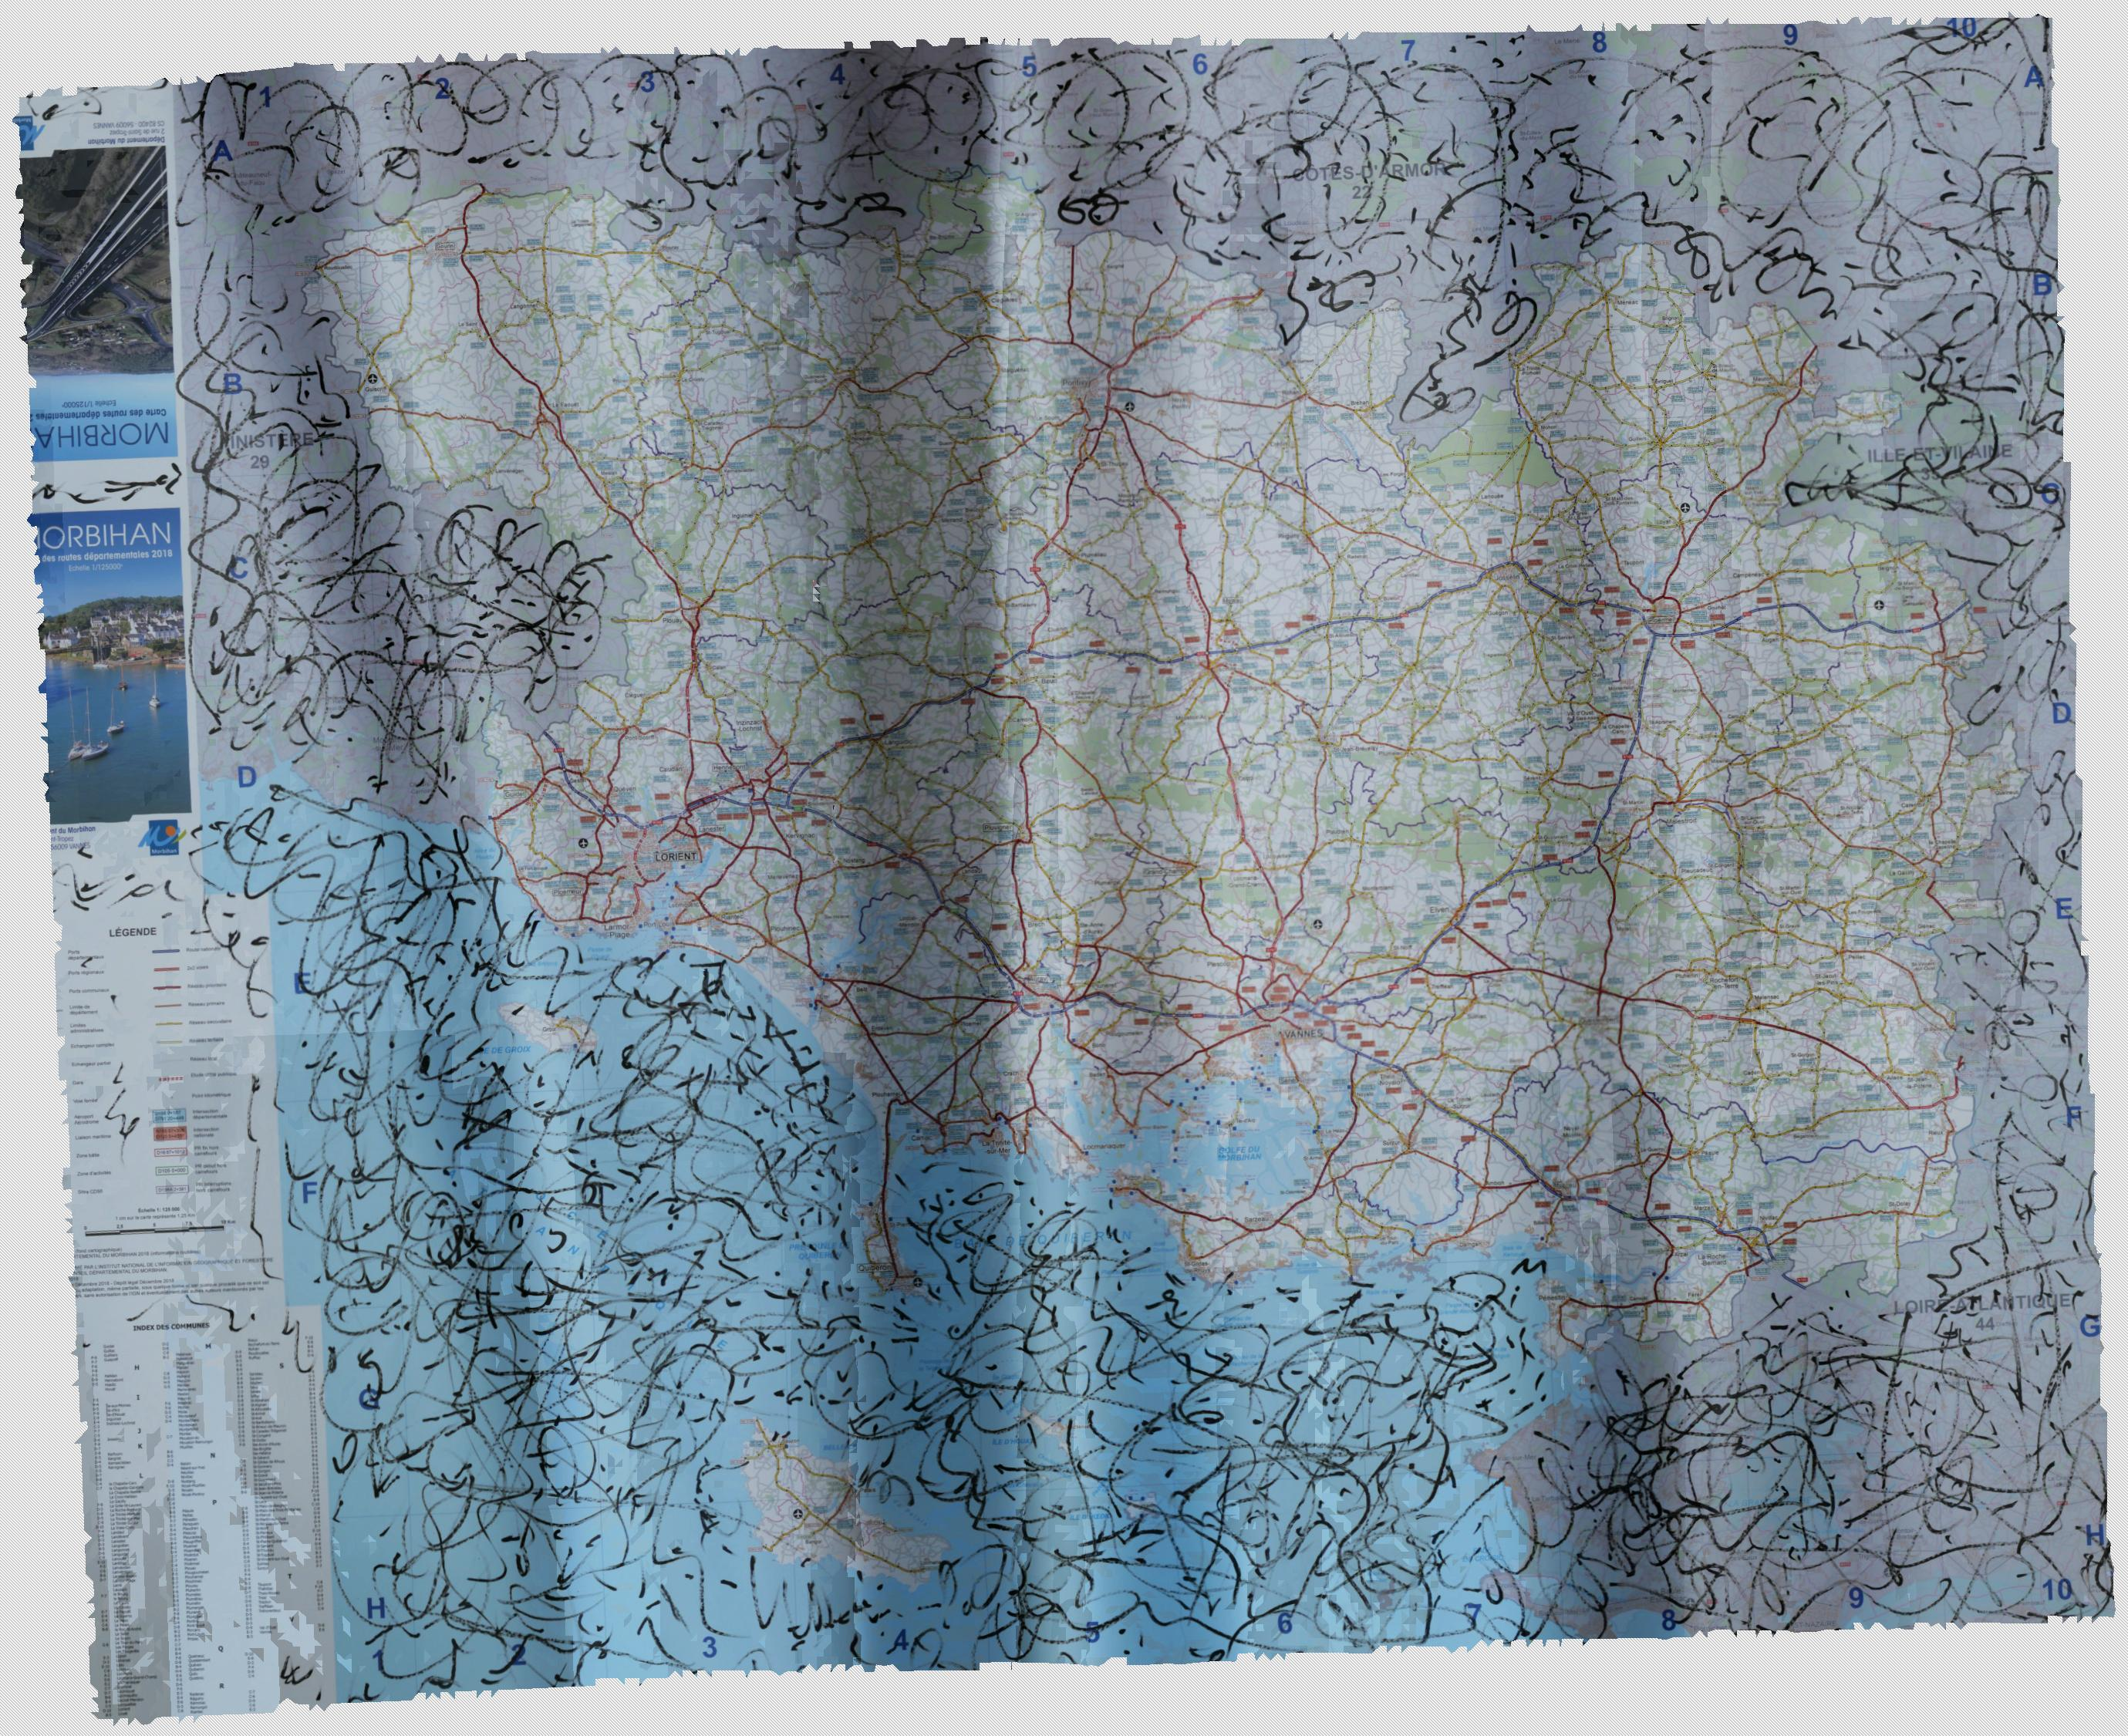
\includegraphics[width=12 cm]{Tutorial/Images/DevIm.jpg}
	\caption{Example of devloped image}
\label{fig:TutDI:DevIm}
\end{figure}



%   ------------------------------------------------------------------
%   ------------------------------------------------------------------
%   ------------------------------------------------------------------

\section{Coded target processing}

%   ------------------------------------------------------------------

\subsection{Introduction/presentation}

This data set, located on {\tt Circ-Code-Target} is representative of an acquisition specially made for close 
range calibration of a camera, or block rigid camera.  The images have been
acquired on specially build camera panel ; the caracteristics of this panel
is the following (see an example on figure~\ref{fig:CodeT:Panel}) :
 

\begin{itemize}
     \item it contain arround $234$ targets, which $3d$ position has been accurately measured;

     \item arround $\frac{1}{4}$ of these targets are coded target that allow a firt full automatic pipeline,
           while the non coded target can  be automatically matched in a second iteration;

     \item for easiness of conception,  the majority of the points are in a plane, by the way $3$ target
           are outside the plane  to offer a better calibration of the focal length;
\end{itemize}


\begin{figure}
\centering
	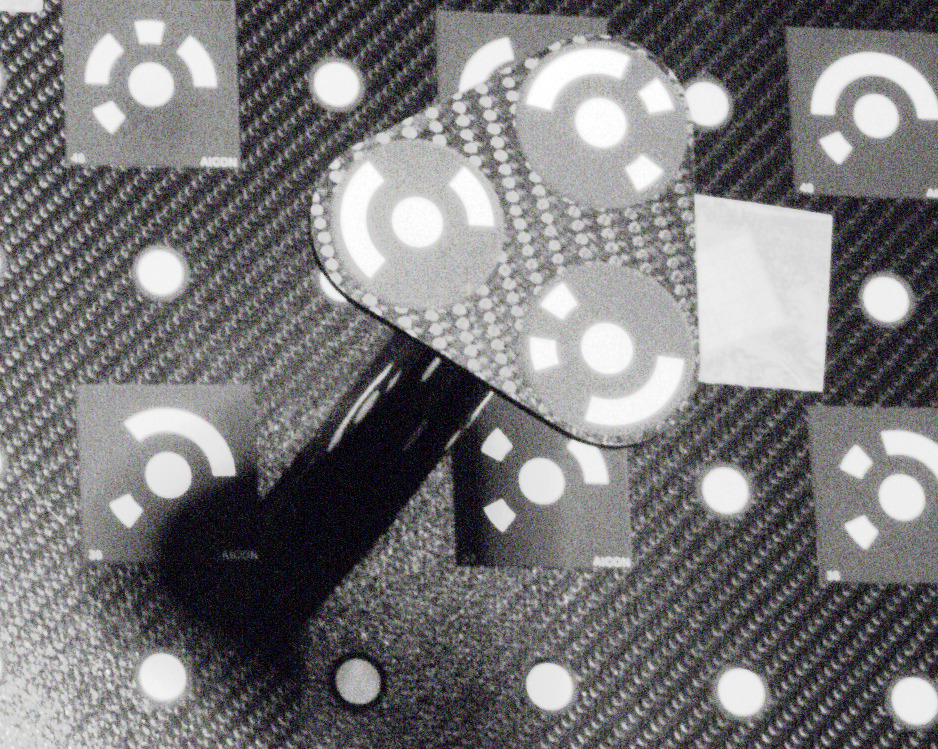
\includegraphics[width=5cm]{Tutorial/Images/Perche.jpg}
	\caption{An extract of panel including the $3$ foreground target.}
\label{fig:CodeT:Panel}
\end{figure}


The acquisition system initially contain $4$ camera in a rigid block position, each camera acquired
$40$ images of $6000 \times  4000$ pixels. For limiting the size of data on github, the following reduction
where applied : limitation to $2$ camera, $20$ images per camera and downsizing the image to $2000 \times  1333$ pixels

The images contain no meta-data, but we "know" that :

\begin{itemize}
     \item the camera model is a Nikon D5600 ;
     \item the focal lenght is a $24mm$, in equivalent $35mm$ (in fact a $16mm$);
     \item different instance of the same camera have been used in the rigid
           block, the $3$ first digit of image name can be used as identifier
           (i.e. two images have been acquired with the same camera iff their name have the
		same $3$ first digit);
\end{itemize}


%   ------------------------------------------------------------------

\subsection{Extract the target in image}

     %   -  -  -  -  -  -  -  -  -  -  -  -  -  -  -  -  -  -  -  -  -  -  -  -

\subsubsection{Create specification}

{\tt MMVII} offers a flexible way to specify coding system (see \ref{GenEncodS}) :
number of bits, redundancy,  maximal run, geometry ... By the way, here we use
an existing system, so we have no flexibility and just have to specify the reference 
of this system.  Using the general formalism, we do it in two steps, first generate
the encoding, i.e. the set of bit-vector :

\begin{lstlisting}
MMVII  CodedTargetGenerateEncoding CERN 14
\end{lstlisting}

The command generate a file {\tt CERN\_Nbb14\_Freq14\_Hamm1\_Run1000\_1000\_SpecEncoding.xml}
that contains the list of code used. An extract :

\begin{lstlisting}
...
     <el>  <!--10110001000000-->
            <NumCode>4 141</NumCode>
            <Name>"004"</Name>
     </el>
...
\end{lstlisting}

A quick command on the file :

\begin{itemize}
	\item the vector of bit, on $14$ bits  {\tt "10110001000000"} is indicated
		as  commentary (only for ;
        \item it correspond to$128+8+4+1=141$, this is $141$ which is saved
		and used by {\tt MMVII} to compute the bit vvect
	\item  the  number $4$ will be used as identifier  (it's the number printed on the targets);
	\item  the  name {\tt "004"} is the string version.
\end{itemize}

After we generate a file that contains the complete specification : the coding itself
\emph{and} the aspect of the target : geometry and radiometry .  Here again
as we use an existing external system, we dont change anything to default parameters.

\begin{lstlisting}
MMVII  CodedTargetGenerate  CERN_Nbb14_Freq14_Hamm1_Run1000_1000_SpecEncoding.xml
\end{lstlisting}

In case we want to generate an image of the targets (for printing them) we can
use the optionnal parameter {\tt PatIm}.

\begin{lstlisting}
MMVII  CodedTargetGenerate  CERN_Nbb14_Freq14_Hamm1_Run1000_1000_SpecEncoding.xml  PatIm=001
\end{lstlisting}

     %   -  -  -  -  -  -  -  -  -  -  -  -  -  -  -  -  -  -  -  -  -  -  -  -

\subsubsection{Extract the target}

We can now run the extraction of target in image :

\begin{lstlisting}
MMVII  CodedTargetCircExtract 043_0005_Scaled.tif CERN_Nbb14_Freq14_Hamm1_Run1000_1000_FullSpecif.xml DiamMin=8
\end{lstlisting}

Note the parameter {\tt DiamMin=8} necessary here because downscaling has created relatively small targets. 
The result are written in a subfolder of {\tt MMVII-PhgrProj/PointsMeasure/}, by default it's the subfolder
{\tt Std/}, that contains now $2$ files :

\begin{itemize}
	\item {\tt MesIm-043\_0005\_Scaled.tif.xml} that contains the position of the targets, used in standard process;
	\item {\tt Attribute-MesIm-043\_0005\_Scaled.tif.xml} that contains the geometry of ellipses (used in completion/refinement);
\end{itemize}


If we want to check the result we can add the parameter {\tt VisuEllipse=1} to generate an image
including the exracted coded and uncoded targets :


\begin{lstlisting}
MMVII  CodedTargetCircExtract 043_0005_Scaled.tif CERN_Nbb14_Freq14_Hamm1_Run1000_1000_FullSpecif.xml  DiamMin=8 VisuEllipse=1
\end{lstlisting}

An example of result is shown on figure~\ref{fig:CodeT:Panel}.

\begin{figure}
\centering
	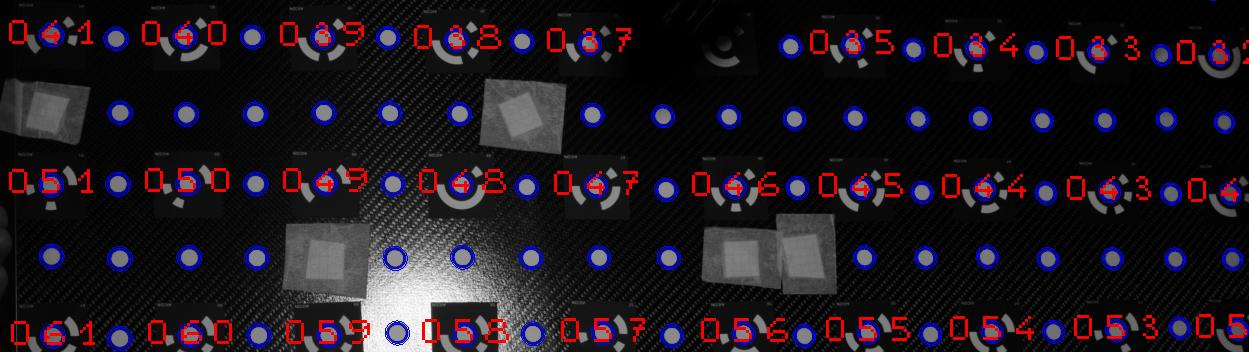
\includegraphics[width=12 cm]{Tutorial/Images/VisuEllips.jpg}
	\caption{An example of the visualization generated}
\label{fig:CodeT:Panel}
\end{figure}

It's possible, to change the destination of result using parameter {\tt OutPointsMeasure}.
Using pattern, its possible to run the research on all the image of the dataset, computation will be parelized .
Like every command {\tt MMVII}, it's possible to restrict the number of processor using the optionnal parameter
{\tt NbProc} :

\begin{lstlisting}
MMVII  CodedTargetCircExtract ".*_Scaled.tif" CERN_Nbb14_Freq14_Hamm1_Run1000_1000_FullSpecif.xml DiamMin=8 NbProc=2 OutPointsMeasure=Test
\end{lstlisting}


%   ------------------------------------------------------------------

\subsection{Estimate pose and calibration simultenaously}

     %   -  -  -  -  -  -  -  -  -  -  -  -  -  -  -  -  -  -  -  -  -  -  -  -

\subsubsection{For one camera}

We can use the command {\tt OriPoseEstim11P} to estimate simultaneously internal and external
calibration:

\begin{lstlisting}
MMVII  OriPoseEstim11P 043_0005_Scaled.tif Test 11P
\end{lstlisting}

It will fail because {\tt MMVII} cannot find the $3d$ measurement of points. They 
have to be located in the same folder than $2d$ measurement of images.
These measures are stored in folder {\tt DataAux}, so we have first to do
something like :

\begin{lstlisting}
cp Data-Aux/MesGCP-AICON-CERN-Pannel.xml MMVII-PhgrProj/PointsMeasure/Test/
\end{lstlisting}

And now we can write again:

\begin{lstlisting}
MMVII  OriPoseEstim11P 043_0005_Scaled.tif Test 11P
\end{lstlisting}

We obtain the result in folder {\tt MMVII-PhgrProj/Ori/11P/} :

\begin{itemize}
	\item {\tt Calib-PerspCentral-043\_0005\_Scaled.tif.xml} contains the internal calibration estimated;
	\item {\tt Ori-PerspCentral-043\_0005\_Scaled.tif.xml} contains the pose estimated, plus a reference to internal calibration.
\end{itemize}

\label{Resec1PPPerIm}

     %   -  -  -  -  -  -  -  -  -  -  -  -  -  -  -  -  -  -  -  -  -  -  -  -

\subsubsection{For several camera (with linear model)}

We can naturally run with several images :

\begin{lstlisting}
MMVII  OriPoseEstim11P .*\_Scaled.tif Tes 11P DoMedianCalib=false
\end{lstlisting}

Note the parameter {\tt DoMedianCalib=false}. By default, if we run  {\tt OriPoseEstim11P}
with several camera, {\tt MMVII} try to compile an internal camera that is some median of 
all the parameter extracted on different camera.  If we do this, to save the result, {\tt MMVII}
will try to compute the standard naming convention that use the focal length and
the name of the camera, if these information are not present we will have an error.

\begin{lstlisting}
MMVII  OriPoseEstim11P .*_Scaled.tif Test 11P

...
=>  Mes=[Camera Name is not init for 043_0005_Scaled.tif]
...
\end{lstlisting}


The problem here is that there is no meta-data {\tt xif} information in the images , so we have to
create a {\tt CalcMTD.xml} to indicate the missing information.
Here we give a easy way to do it because we provide an example file : 

\begin{lstlisting}
cp Data-Aux/CalcMTD.xml  MMVII-PhgrProj/MetaData/Std
\end{lstlisting}

In the case, where there is no data provided, it's also possible t create the file
using the command {\tt EditCalcMTDI} :

\begin{lstlisting}
MMVII EditCalcMTDI Std ModelCam ImTest=043_0005_Scaled.tif  Modif=[.*_Scaled.tif,"NIKON D5600",0] Save=1
MMVII EditCalcMTDI Std Focalmm ImTest=043_0005_Scaled.tif  Modif=[.*_Scaled.tif,24,0] Save=1
MMVII EditCalcMTDI Std AdditionalName ImTest=043_0005_Scaled.tif  Modif=["(.*)_.*_.*","\$1",0] Save=1
\end{lstlisting}

Not the fiedl {\tt AdditionalName} that will allow to make a distinction between group of
images "043.*" and group "671.*" ; this is because
they correspond to two different instances of the same model of camera and focal, current meta data would
not be sufficient to distinguish them.

Now it works :

\begin{lstlisting}
MMVII  OriPoseEstim11P .*_Scaled.tif Test 11P
\end{lstlisting}

We obtain now three kind of result in folder {\tt 11P}:

\begin{itemize}
	\item files with names like  {\tt Calib-PerspCentral-043\_0009\_Scaled.tif.xml} :  internal calibration per images

	\item files with  names like {\tt Ori-PerspCentral-043\_0009\_Scaled.tif.xml} they contain the pose and
		a reference (name) of the internal calibration per images;

	       these two file have already been seen in section~\ref{Resec1PPPerIm}, we have as many such files
               than number of images;


	\item files with  names like {\tt CalibIntr\_CamNIKON\_D5600\_Add043\_Foc24.xml}, these file  are calibration
              per camera;  we see that their name contains the exact information that is required to distinguish between 
              separate camera : focal, model of camera, additional name ({\tt Add043});

\end{itemize}

     %   -  -  -  -  -  -  -  -  -  -  -  -  -  -  -  -  -  -  -  -  -  -  -  -

\subsubsection{Restricting the data-set}

If we look at messages printed, we see that the majority
of images have a focal arround $2700$ , but there are several
outliers :

\begin{lstlisting}
...
NIIII  043_0031_Scaled.tif F=32.1533
...
NIIII  671_0013_Scaled.tif F=124.753
NIIII  671_0025_Scaled.tif F=141.9
NIIII  671_0031_Scaled.tif F=20.6496
\end{lstlisting}


This false estimation are easy to explain , these image contains none of the target that are outside
the plane, and the plane, and are degenerate case for the $11$ parameter algorithm,
as illustrated on figure~\ref{fig:CodeT:DegenCase}.

\begin{figure}
\centering
	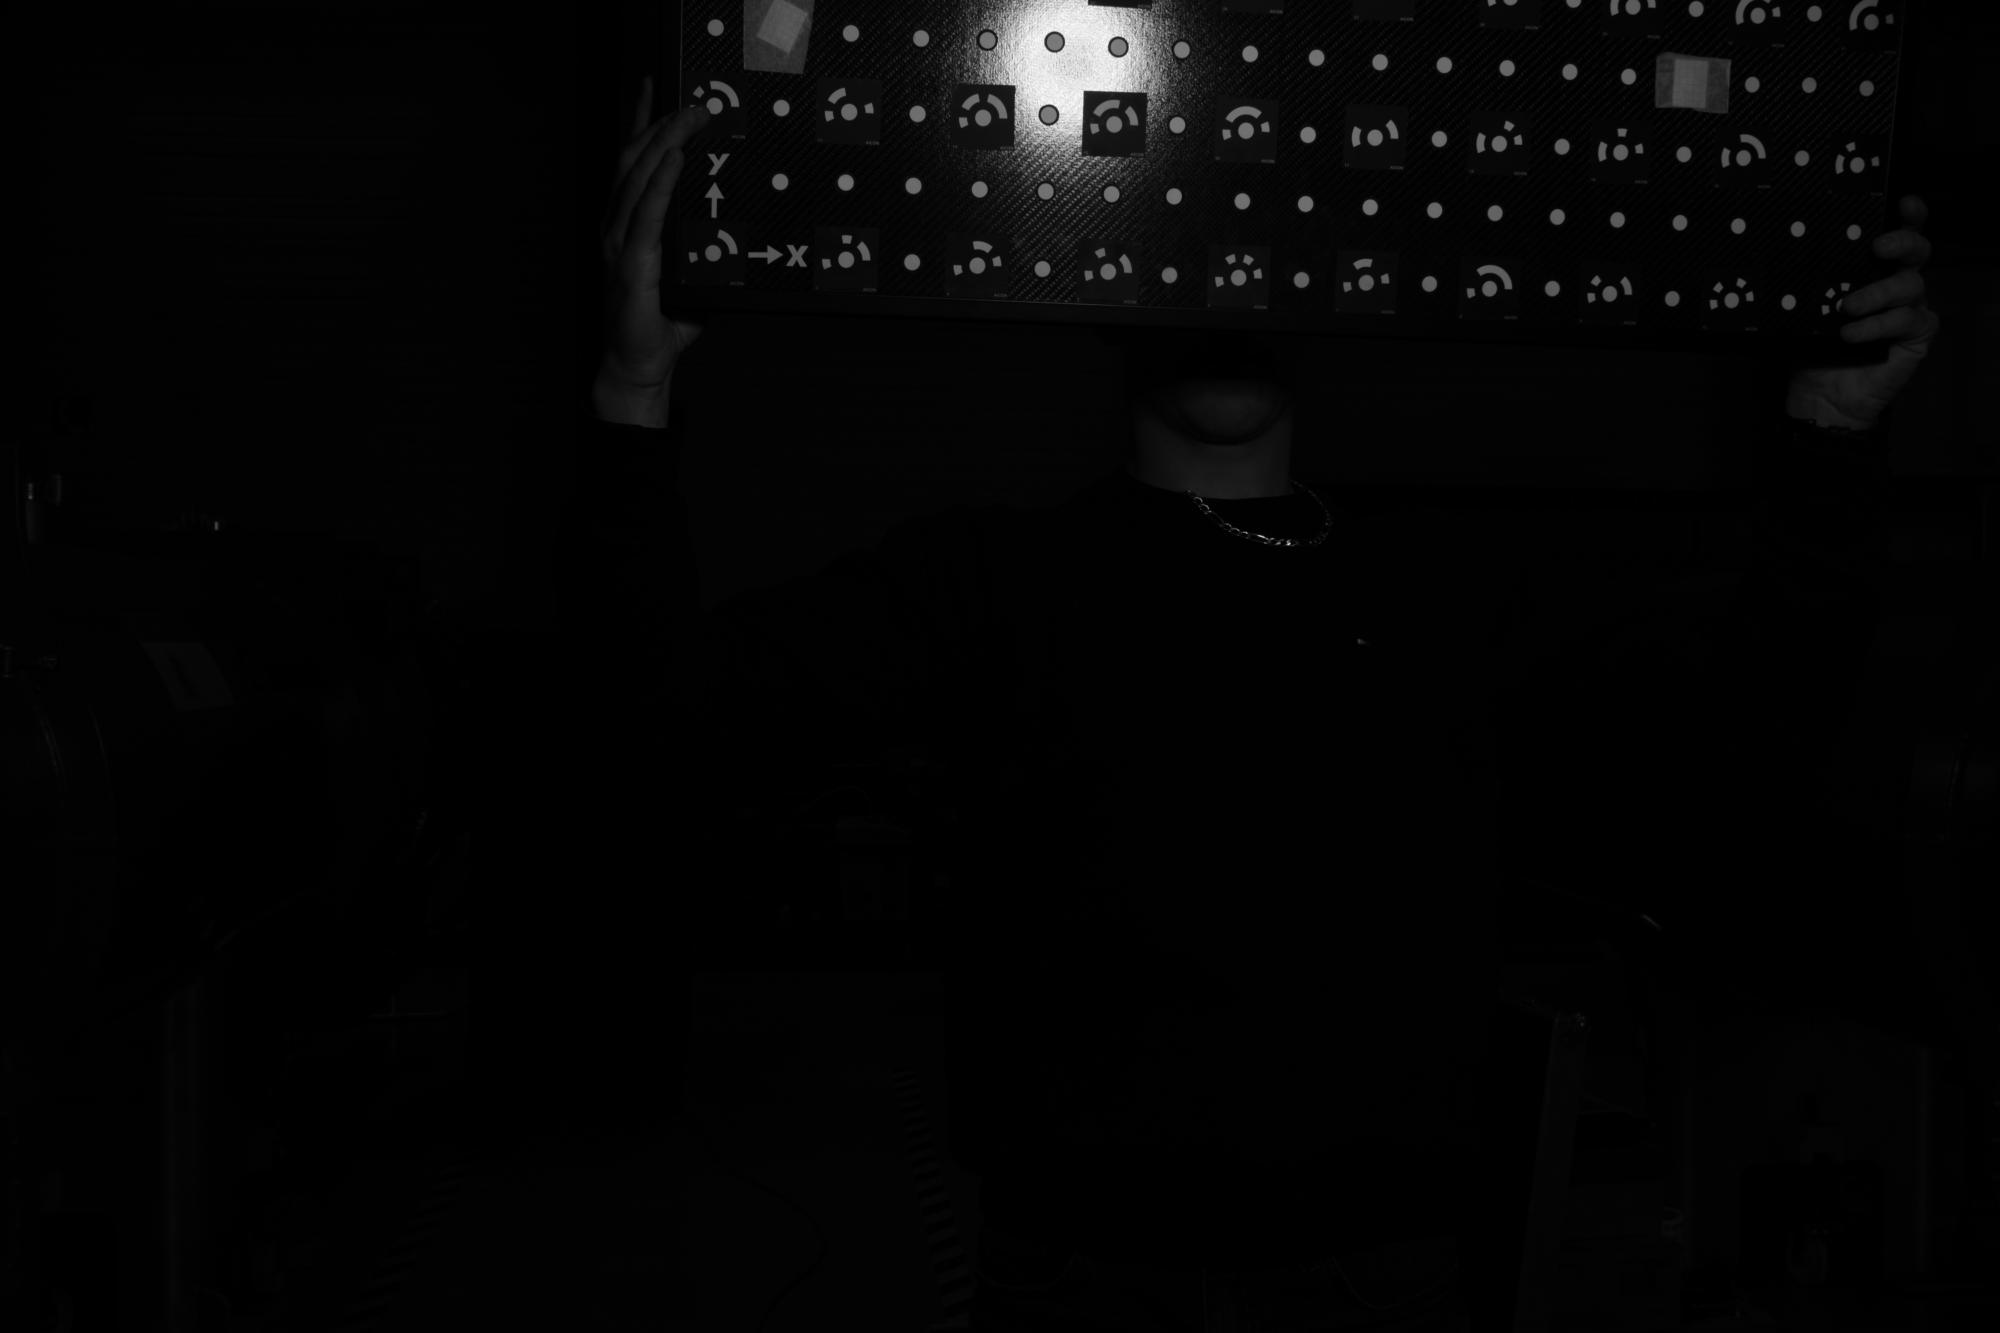
\includegraphics[width=12 cm]{Tutorial/Images/ImageBug.jpg}
	\caption{An image with no 3d target, leading to a degenerate estimation}
\label{fig:CodeT:DegenCase}
\end{figure}

To have a better statibility it's probably a good idea to use only a subset of images
excluding these images. This can be done whith the help of the {\tt EditSet} command.  First
we create a file containing all the images :

\begin{lstlisting}
MMVII EditSet  ImOk.xml = ".*Scaled.tif"
\end{lstlisting}

Then we subsract the images potentially dangerous :

\begin{lstlisting}
MMVII EditSet ImOk.xml -=  043_0031_Scaled.tif
MMVII EditSet ImOk.xml -=  671_0013_Scaled.tif
MMVII EditSet ImOk.xml -=  671_0025_Scaled.tif
MMVII EditSet ImOk.xml -=  671_0031_Scaled.tif
\end{lstlisting}

We can now use {\tt ImOk.xml} instead of a pattern :

\begin{lstlisting}
MMVII  OriPoseEstim11P ImOk.xml Test 11P
\end{lstlisting}

     %   -  -  -  -  -  -  -  -  -  -  -  -  -  -  -  -  -  -  -  -  -  -  -  -

\subsubsection{Estimate distorsion}

It's also possible to estimate some non linear distorsion, they will be
estimated by bundle adjsustment. We cannont expect it to be  very accurate,
by the way as we make a median of all parameter we can hope to have 
avoid "gross  error".

With a standard phorogrammetric model :

\begin{lstlisting}
MMVII  OriPoseEstim11P ImOk.xml Test 11P DegDist=[3,1,1]
\end{lstlisting}

Or with no distorsion :

\begin{lstlisting}
MMVII  OriPoseEstim11P  ImOk.xml Test 11P DegDist=[0,0,0]
\end{lstlisting}

It's also possible to froze a subset of distorsion parameters 

\begin{lstlisting}
MMVII  OriPoseEstim11P  ImOk.xml Test 11P DegDist=[3,1,1] PatFrozen="(b|p).*|K3"
\end{lstlisting}

%   ------------------------------------------------------------------

\subsection{Estimate pose with known calibration}

Once we have estimated an acceptable initial value for internal 
calibration, we can use it for estimating the pose of all images :
we can also use image with all target in a plane, the result is stable
because we dont re-estimate the calibration.

\begin{lstlisting}
MMVII OriPoseEstimSpaceResection .*Scaled.tif Test 11P  Resec
\end{lstlisting}

In folder {\tt Resec} we see that we have only the $2$ internal calibration
that depend from camera and that the file for pose refers to these calibration.
Now that we have a calibration shared by all images taken by the same camera, and 
poses that have been computed with these calibration, we are ready to make
a real bundle adjustment :


\begin{lstlisting}
MMVII OriBundleAdj ".*_Scaled.tif" Resec BA  GCPW=[1,1] DataDir=Test
\end{lstlisting}

%   ------------------------------------------------------------------

\subsection{Complete the target}

Now that we have computed reliable  orientation, we can use it to identify and
validate the uncoded targets :

\begin{lstlisting}
MMVII CodedTargetCompleteUncoded .*_Scaled.tif BA 1.0 InPointsMeasure=Test
\end{lstlisting}

All the measure are stored in the  folder {\tt Completed} (by default). We can make a
bundle adjustment with these new measures :

\begin{lstlisting}
MMVII OriBundleAdj ".*_Scaled.tif"  BA BA2  GCPW=[1,1] DataDir=Completed
\end{lstlisting}




\section{Clinometers calibration processing}

\subsection{Introduction}

This section presents how to add clinometers to an image orientation. You are supposed to have :
\begin{itemize}
     \item a calibrated camera
     \item a set of images
     \item a set of measures acquired by clinometers in the same time than images
     \item a set of GCP points
\end{itemize}

The relative orientation between camera to the clinometers are supposed to be constant through all acquisitions.
The aim of this calibration is to compute the relative orientations (Boresight matrixes) between camera and each clinometers.

In a first step, an approximation of these Boresight matrixes are computed with {\tt ClinoInit}. 
In a second step, these Boresight matrixes are computed with bundle adjustment with {\tt OriBundleAdj}.


\subsection{Equations}

Two equations are used for bundle adjustment :
\begin{itemize}
     \item the first one uses only one clinometer and determines its Boresight matrix
     \item the second one uses two clinometers and checkes that their relative orientation is almost the same than their initial relative orientation. 
     This equation prevents the least squares from diverging
\end{itemize}


$R_C$ is the rotation of the camera in the absolute system.\\

$B_1$ is the first Boresight matrix : the rotation from camera system to first clinometer system. $B_{10}$ is the initial approximation of $B_1$.

$B_2$ is the second Boresight matrix : the rotation from camera system to second clinometer system. $B_{20}$ is the initial approximation of $B_2$.

$B_1$ and $B_2$ are the unknowns of the problem.\\

The first clinometer measure is $\theta_1$. 

The second clinometer measure is $\theta_2$. \\

For each clinometer, $(\Vec{i}, \Vec{j}, \Vec{k})$ is the clinometer system and $\theta$ is the measure of angle between $\Vec{i}$ and the vertical in the plan $(\Vec{i}, \Vec{j})$.

The vertical in the local system is $ \Vec{v_{loc}} $ \\


\subsubsection{First equation}

\label{FirstClinoCalibEq}


The vertical in the camera system is $ R_C \Vec{v_{loc}} $

The vertical in the first clinometer system is $\Vec{v_{clino}} = B_1 R_C \Vec{v_{loc}} $\\

Each clinometer gives the angle between the vertical and one plan of its system.

$\Phi$ is the projection of a vector on the plan $(\Vec{i}, \Vec{j})$ :
\begin{equation}
     \Phi \begin{pmatrix}
          v_i \\
          v_j \\
          v_k
     \end{pmatrix} = \begin{pmatrix}
          v_i \\
          v_j
     \end{pmatrix}
\end{equation}


Finally :
\begin{equation}
     \frac{\Phi (\Vec{v_{clino}})}{|| \Phi (\Vec{v_{clino}}) ||}   = \begin{pmatrix}
          cos(\theta_1) \\
          sin(\theta_1)
     \end{pmatrix}
\end{equation}


\subsubsection{Second equation}

\label{SecondClinoCalibEq}

This equation is not mathematically exact but prevents the least square from diverging : relative orientation between couple of clinometers are supposed to be constant in the time.

\begin{equation}
     B_2 B_1^\intercal = B_{20} B_{10}^\intercal
\end{equation}

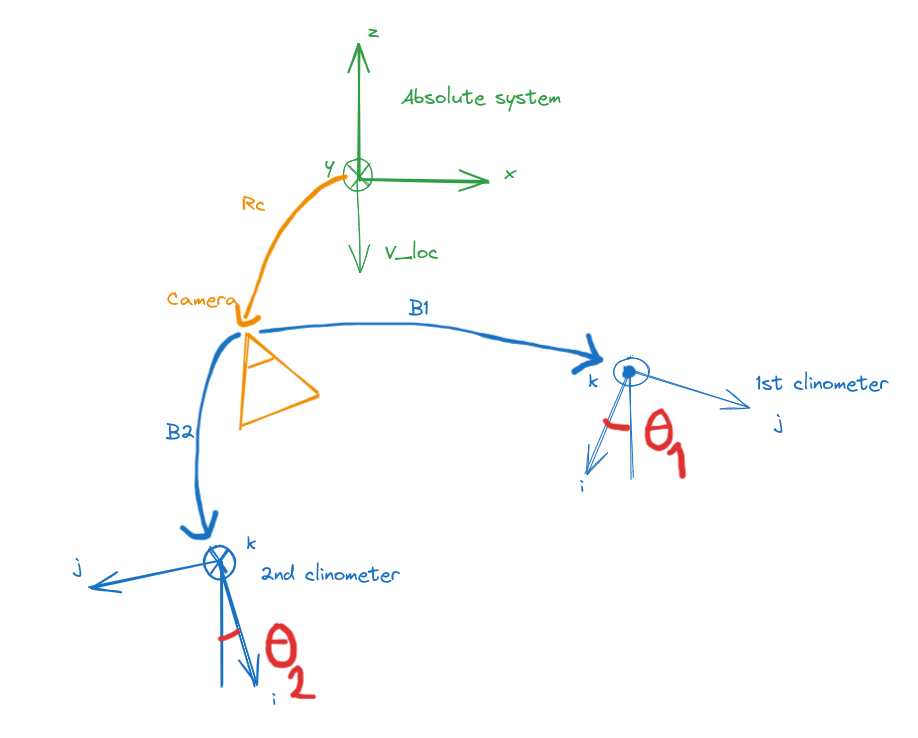
\includegraphics[width=12cm]{Programmer/ClinoBA.png}


\subsection{Clinometers measures file}

The file with clinometers measures must have :
\begin{itemize}
     \item one line per camera
     \item in each line, the image name
     \item in each line, the measures of the two clinometers
     \item each clinometer measure has the name of the clinometer, its measure and its sigma  
\end{itemize}

For example, the file should be like :

\begin{lstlisting}
image1 clino1 +0.064786 +0.00001 clino2 +0.014629 +0.00002
image2 clino1 +0.064786 +0.00001 clino2 +0.014629 +0.00002
image3 clino1 +0.064786 +0.00001 clino2 +0.014629 +0.00002
\end{lstlisting}



\subsection{ClinoInit}

The first step is to find approximation of the Boresight matrixes with {\tt ClinoInit}.

\begin{lstlisting}
     MMVII ClinoInit Data-Input/ClinoMeasures.txt "ISF#SF#" [1,0] BA_Clino_B  INIT_CLINO Rel12="i-kj" OkNoCam=true PrePost=[949_,.JPG]
\end{lstlisting}


Parameters of {\tt ClinoInit} are :
\begin{itemize}
     \item Data-Input/ClinoMeasures.txt : file with clinometers measures.
     \item "ISF\#SF\#" : structure of ClinoMeasures.txt : I for image name, S for clinometer name, F for a value, \# for a not used column. In {\tt ClinoInit}, sigma are not used
     \item $[$1,0$]$ : index of clinometers in ClinoMeasures.txt
     \item BA$\_$Clino$\_$B : orientation of camera
     \item INIT$\_$CLINO : name of directory where approximation of clinometers calibrations will be saved
     \item Rel12="i-kj" : an approximation of the relative orientation between the two clinometers systems ($\Vec{i_2}=\Vec{i_1}, \Vec{j_2}=-\Vec{k_1}, \Vec{k_2}=\Vec{j_1}$)
     \item OkNoCam=true : if true, do not raise error if an image in ClinoMeasures.txt is not in BA$\_$Clino$\_$B
     \item PrePost=[949$\_$,.JPG] : values added before and after image names in ClinoMeasures.txt to have the same names than in BA$\_$Clino$\_$B
\end{itemize}

In INIT$\_$CLINO, there are the clinometers name with their approximate Boresight matrix. There is also the approximation of the relative orientation between the two clinometers system.



\subsection{OriBundleAdj}

Then, you can compute the Boresight matrixes with {\tt OriBundleAdj}. You need to complete the parameter NameClino to compute the clinometers calibration

\begin{lstlisting}
     MMVII  OriBundleAdj  AllImClino.xml  BA_Clino_B   BA_Clino_C   GCPDir=ClinoCompl  GCPW=[1,1,0.5]  PPFzCal=.* ClinoDirIn=INIT_CLINO ClinoDirOut=CALIB_CLINO NameClino=Data-Input/ClinoMeasures.txt Format=ISFFSFF PrePost=[949_,.JPG]
\end{lstlisting}

Parameters of {\tt ClinoInit} are :
\begin{itemize}
     \item AllImClino.xml : name of images
     \item BA$\_$Clino$\_$B : orientation of camera
     \item BA$\_$Clino$\_$C : orientation of camera after the bundle adjustment
     \item GCPDir=ClinoCompl : directory for GCP
     \item GCPW=[1,1,0.5] : GCP weights
     \item PPFzCal=.* : freeze internal calibration
     \item ClinoDirIn=INIT$\_$CLINO : approximation of the two Boresight matrixes computed with {\tt ClinoInit}
     \item ClinoDirOut=CALIB$\_$CLINO : name of directory where clinometers calibrations will be saved
     \item NameClino=Data-Input/ClinoMeasures.txt : file with clinometers measures.
     \item "ISFFSFF" : structure of ClinoMeasures.txt. This time, sigmas are used
     \item PrePost=[949$\_$,.JPG] : see {\tt ClinoInit}
\end{itemize}

The output clinometers orientations are the same than for {\tt ClinoInit}.
